\section{Vector-Valued Functions}

\subsection{Coordinate Systems in 3D Space}

Specifying a point or giving directions in space can be accomplished in multiple ways:
\begin{itemize}
    \item Giving a direction and a distance.
    \item Using Cartesian coordinates $(d_1, d_2, d_3) = (x, y, z)$.
    \item Specifying an angle relative to a reference axis along with a magnitude.
    \item Referencing a relative landmark.
    \item Using geographic coordinates like latitude and longitude.
\end{itemize}

\subsubsection{Polar Coordinates (2D)}
In the $xy$-plane, a point is specified by its radial distance $r$ from the origin and an angle $\theta$ relative to the positive $x$-axis: $(r, \theta)$.

\[
r = \sqrt{x^2 + y^2} \quad (r \ge 0)
\]

While $\theta = \arctan\left(\frac{y}{x}\right)$ is commonly used, it is undefined when $x = 0$. The foundational algebraic transformation between systems is given by:
\begin{align*}
x &= r\cos\theta \\
y &= r\sin\theta
\end{align*}


\subsubsection{Cylindrical Coordinates}
Cylindrical coordinates $(r, \theta, z)$ extend polar coordinates into 3D space by preserving the standard Cartesian $z$-axis:
\begin{align*}
x &= r\cos\theta \\
y &= r\sin\theta \\
z &= z
\end{align*}

\subsubsection{Spherical Coordinates}
Spherical coordinates are represented as $(\rho, \theta, \phi)$, where $\rho$ is the distance from the origin, $\theta$ is the azimuthal angle in the $xy$-plane, and $\phi$ is the polar angle measured down from the positive $z$-axis.

\begin{align*}
x &= \rho\sin\phi\cos\theta \\
y &= \rho\sin\phi\sin\theta \\
z &= \rho\cos\phi
\end{align*}

The standard domain boundaries are:
\begin{align*}
\rho &\ge 0 \\
0 &\le \theta < 2\pi \\
0 &\le \phi \le \pi
\end{align*}

\begin{center}
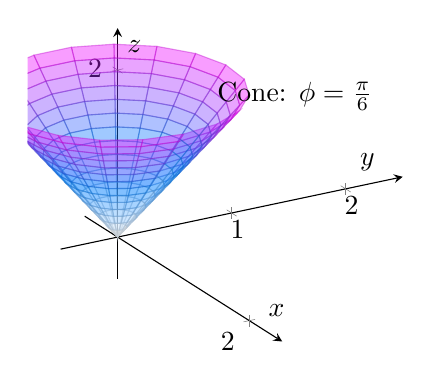
\begin{tikzpicture}
\begin{axis}[
    view={60}{30},
    axis lines=center,
    xlabel={$x$}, ylabel={$y$}, zlabel={$z$},
    xmin=-0.5, xmax=2.5, ymin=-0.5, ymax=2.5, zmin=-0.5, zmax=2.5
]
    % Cone for phi = pi/6
    \addplot3[surf, domain=0:2, domain y=0:360, samples=15, samples y=20, variable=\r, variable y=\t, opacity=0.4, colormap/cool]
        ({r*sin(30)*cos(t)}, {r*sin(30)*sin(t)}, {r*cos(30)});
    \node[anchor=south west] at (axis cs: 0.5,0.5,1.5) {Cone: $\phi = \frac{\pi}{6}$};
\end{axis}
\end{tikzpicture}
\end{center}

\subsection{Coordinate System Transformations}

\begin{problem}{Conversion Between Coordinate Systems}{conversion_between_coordinate_systems}
Convert the surface equation $x^2 + \dfrac{y^2}{a^2} = z^2$ into cylindrical and spherical coordinates.
\end{problem}

\begin{sol}
\textbf{Cylindrical Coordinates:} \\
Substituting $x = r\cos\theta$, $y = r\sin\theta$, and $z = z$ into the original equation yields:
\begin{align*}
(r\cos\theta)^2 + \frac{(r\sin\theta)^2}{a^2} &= z^2 \\
r^2\cos^2\theta + \frac{r^2\sin^2\theta}{a^2} &= z^2 \\
r^2\left(\cos^2\theta + \frac{\sin^2\theta}{a^2}\right) &= z^2
\end{align*}

\textbf{Spherical Coordinates:} \\
Substituting $x = \rho\sin\phi\cos\theta$, $y = \rho\sin\phi\sin\theta$, and $z = \rho\cos\phi$ into the original equation yields:
\begin{align*}
(\rho\sin\phi\cos\theta)^2 + \frac{(\rho\sin\phi\sin\theta)^2}{a^2} &= (\rho\cos\phi)^2 \\
\rho^2\sin^2\phi\cos^2\theta + \frac{\rho^2\sin^2\phi\sin^2\theta}{a^2} &= \rho^2\cos^2\phi \\
\rho^2\sin^2\phi\left(\cos^2\theta + \frac{\sin^2\theta}{a^2}\right) &= \rho^2\cos^2\phi
\end{align*}
Assuming $\rho \neq 0$, we divide both sides by $\rho^2$:
\begin{align*}
\sin^2\phi\left(\cos^2\theta + \frac{\sin^2\theta}{a^2}\right) &= \cos^2\phi \\
\cos^2\theta + \frac{\sin^2\theta}{a^2} &= \frac{\cos^2\phi}{\sin^2\phi} \\
\cos^2\theta + \frac{\sin^2\theta}{a^2} &= \cot^2\phi
\end{align*}
\end{sol}

\subsection{Vector-Valued Functions}

\begin{definition}{Vector-Valued Functions}{vector_value_functions}
A vector-valued function maps one or more real parameters to a space vector:
\[
\vv{r}(t) = \ang{x(t), y(t), z(t)}, \quad \vv{r}: I \rightarrow \mathbb{R}^3
\]
where $I \subseteq \mathbb{R}$ is an interval. This traces out a spatial curve parametrized by $t$.
\end{definition}

\begin{example}
Consider the vector function $\vv{r}(t) = \ang{\cos t, \sin t, 1}$ for $0 \le t < 2\pi$. This describes a unit circle in 3D space elevated to the horizontal plane $z = 1$.

\begin{center}
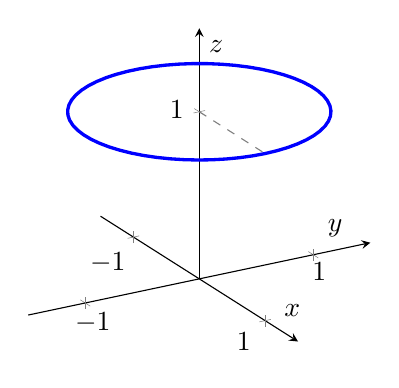
\begin{tikzpicture}
\begin{axis}[
    view={60}{30},
    axis lines=center,
    xlabel={$x$}, ylabel={$y$}, zlabel={$z$},
    xmin=-1.5, xmax=1.5, ymin=-1.5, ymax=1.5, zmin=0, zmax=1.5
]
    \addplot3[domain=0:360, samples=60, samples y=0, line width=1.2pt, blue]
        ({cos(x)}, {sin(x)}, {1});
    \draw[dashed, gray] (axis cs: 0,0,1) -- (axis cs: 1,0,1);
\end{axis}
\end{tikzpicture}
\end{center}
\end{example}

\begin{problem}{Finding Collisions and Intersections}{finding_collisions}
Let $\vv{r}_1(t) = \ang{t^2 + \dfrac{t}{2}, t - t^3}$ and $\vv{r}_2(t) = \ang{t, t^2}$. Find all collision points and structural intersections between the curves.
\end{problem}

\begin{sol}
\textbf{1. Collision Points (Same location at same time $t$):} \\
Setting $\vv{r}_1(t) = \vv{r}_2(t)$ gives:
\begin{align*}
\ang{t^2 + \dfrac{t}{2}, t - t^3} &= \ang{t, t^2}
\end{align*}
Equating the individual components gives the system:
\begin{align*}
t^2 + \frac{t}{2} &= t \\
t - t^3 &= t^2
\end{align*}
Solving the first equation for $t$:
\begin{align*}
t^2 + \frac{t}{2} - t &= 0 \\
t^2 - \frac{t}{2} &= 0 \\
t\left(t - \frac{1}{2}\right) &= 0 \implies t = 0 \quad \text{or} \quad t = \frac{1}{2}
\end{align*}
Now, we verify both parameters in the second component equation $t - t^3 = t^2$:
\begin{align*}
\text{For } t = 0: \quad 0 - (0)^3 &= (0)^2 \implies 0 = 0 \quad \text{(Valid)} \\
\text{For } t = \frac{1}{2}: \quad \frac{1}{2} - \left(\frac{1}{2}\right)^3 &= \frac{1}{2} - \frac{1}{8} = \frac{3}{8} \\
\left(\frac{1}{2}\right)^2 &= \frac{1}{4} = \frac{2}{8} \neq \frac{3}{8} \quad \text{(Invalid)}
\end{align*}
Therefore, $t = 0$ is the only valid collision time. Evaluating $\vv{r}_1(0)$:
\begin{align*}
\vv{r}_1(0) &= \ang{0^2 + \frac{0}{2}, 0 - 0^3} = \ang{0, 0}
\end{align*}
The collision point is $(0, 0)$.

\textbf{2. Intersection Points (Same location at potentially different times $t$ and $s$):} \\
Setting $\vv{r}_1(t) = \vv{r}_2(s)$ gives:
\begin{align*}
\ang{t^2 + \frac{t}{2}, t - t^3} &= \ang{s, s^2}
\end{align*}
Equating components yields:
\begin{align*}
s &= t^2 + \frac{t}{2} \tag{1} \\
t - t^3 &= s^2 \tag{2}
\end{align*}
Substituting equation (1) into equation (2):
\begin{align*}
t - t^3 &= \left(t^2 + \frac{t}{2}\right)^2 \\
t - t^3 &= t^4 + t^3 + \frac{t^2}{4} \\
0 &= t^4 + 2t^3 + \frac{t^2}{4} - t \\
0 &= t\left(t^3 + 2t^2 + \frac{t}{4} - 1\right)
\end{align*}
Setting each factor to zero:
\begin{align*}
t = 0 & \implies s = 0^2 + \frac{0}{2} = 0 \\
&\implies \text{Intersection point } (0, 0) \\
t^3 + 2t^2 + \frac{t}{4} - 1 = 0 & \implies t \approx 0.576
\end{align*}
Solving for $s$ when $t \approx 0.576$:
\begin{align*}
s &= (0.576)^2 + \frac{0.576}{2} \\
s &\approx 0.332 + 0.288 \approx 0.620
\end{align*}
Evaluating the spatial coordinates using $\vv{r}_2(s)$:
\begin{align*}
x &= s \approx 0.620 \\
y &= s^2 \approx (0.620)^2 \approx 0.384
\end{align*}
Hence, the two spatial intersection points are $(0, 0)$ and $(0.620, 0.384)$.
\end{sol}

\subsection{Gallery of Parametric Space Curves}

Below are standard parametric 3D space curves used in multivariable trajectory analysis:

\begin{center}
\begin{minipage}{0.32\textwidth}
\centering
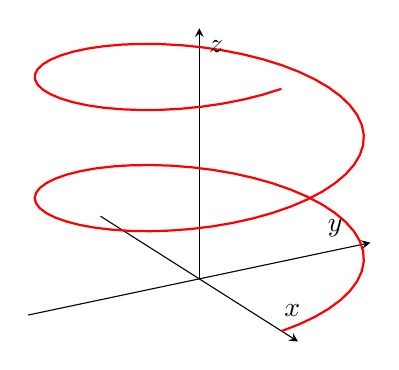
\begin{tikzpicture}
\begin{axis}[
    view={60}{30},
    axis lines=center,
    xlabel={$x$}, ylabel={$y$}, zlabel={$z$},
    xmin=-1.2, xmax=1.2, ymin=-1.2, ymax=1.2, zmin=0, zmax=13,
    ticks=none
]
    \addplot3[domain=0:4*pi, samples=100, samples y=0, thick, red]
        ({cos(deg(x))}, {sin(deg(x))}, {x});
\end{axis}
\end{tikzpicture}
\\[0.5em]
$\vv{r}(t) = \ang{\cos t, \sin t, t}$
\end{minipage}
\hfill
\begin{minipage}{0.32\textwidth}
\centering
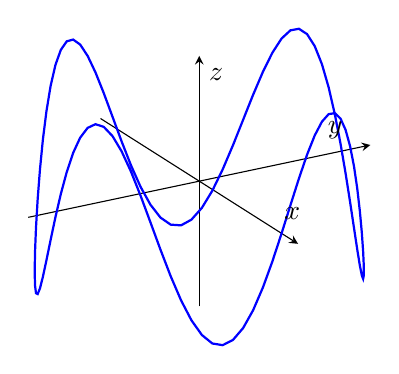
\begin{tikzpicture}
\begin{axis}[
    view={60}{30},
    axis lines=center,
    xlabel={$x$}, ylabel={$y$}, zlabel={$z$},
    xmin=-1.2, xmax=1.2, ymin=-1.2, ymax=1.2, zmin=-1.2, zmax=1.2,
    ticks=none
]
    \addplot3[domain=0:2*pi, samples=100, samples y=0, thick, blue]
        ({cos(deg(x))}, {sin(deg(x))}, {sin(4*deg(x))});
\end{axis}
\end{tikzpicture}
\\[0.5em]
$\vv{r}(s) = \ang{\cos s, \sin s, \sin(4s)}$
\end{minipage}
\hfill
\begin{minipage}{0.32\textwidth}
\centering
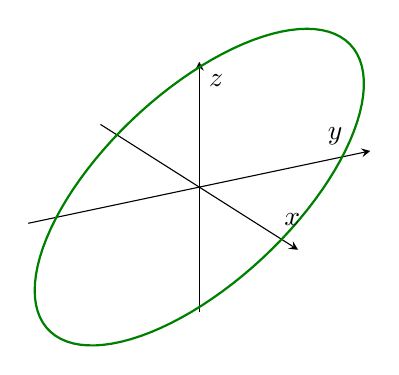
\begin{tikzpicture}
\begin{axis}[
    view={60}{30},
    axis lines=center,
    xlabel={$x$}, ylabel={$y$}, zlabel={$z$},
    xmin=-1.2, xmax=1.2, ymin=-1.2, ymax=1.2, zmin=-4.2, zmax=4.2,
    ticks=none
]
    \addplot3[domain=0:2*pi, samples=100, samples y=0, thick, green!50!black]
        ({cos(deg(x))}, {sin(deg(x))}, {4*sin(deg(x))});
\end{axis}
\end{tikzpicture}
\\[0.5em]
$\vv{r}(t) = \ang{\cos t, \sin t, 4\sin t}$
\end{minipage}
\end{center}

\subsection{Parameterization of Curves and Surfaces}

\begin{problem}{Parameterization of a Curve on a Surface}{parameterization_of_surfaces}
Find a parameterization for the curve given by the intersection of the surfaces $y = \sqrt{x^2 + z^2}$ and $x = z^2$.
\end{problem}

\begin{sol}
Notice that for any choice of $z \in \mathbb{R}$, the value of $x$ is uniquely determined by $x = z^2$. We can set $z = t$ as our parameter.
Then,
\begin{align*}
    x &= t^2 \\
    z &= t \\
    y &= \sqrt{(t^2)^2 + t^2} = \sqrt{t^4 + t^2} = |t|\sqrt{t^2 + 1}
\end{align*}
Thus, a vector parameterization of the curve is:
\[
\vv{r}(t) = \ang{t^2, |t|\sqrt{t^2 + 1}, t}, \quad t \in \mathbb{R}
\]
\end{sol}

\subsection{Calculus of Vector-Valued Functions}

Calculus operations on vector-valued functions are defined component-wise.

For a vector-valued function $\vv{r}(t) = \ang{x(t), y(t), z(t)}$, limits, derivatives, and integrals are computed as follows:

\[
\lim_{t \to t_0} \vv{r}(t) = \ang{\lim_{t \to t_0} x(t), \lim_{t \to t_0} y(t), \lim_{t \to t_0} z(t)}
\]

\[
\vv{r}'(t) = \ang{x'(t), y'(t), z'(t)}
\]

\[
\int_a^b \vv{r}(t) \dd{t} = \ang{\int_a^b x(t) \dd{t}, \int_a^b y(t) \dd{t}, \int_a^b z(t) \dd{t}}
\]

\begin{example}[Tangent Vectors and Parameterizing Tangent Lines]
Given the circular helix $\vv{r}(t) = \ang{\cos t, \sin t, t}$.

Differentiating component-wise gives:
\begin{align*}
\vv{r}'(t) &= \ang{-\sin t, \cos t, 1} \\
\vv{r}'(0) &= \ang{0, 1, 1}
\end{align*}

The derivative $\vv{r}'(0)$ yields a vector representing the tangent direction of the curve at $t = 0$.

\begin{center}
\begin{tikzpicture}
\begin{axis}[
    view={60}{30},
    axis lines=center,
    xlabel=$x$, ylabel=$y$, zlabel=$z$,
    xmin=-1.5, xmax=1.5,
    ymin=-1.5, ymax=1.5,
    zmin=0, zmax=7,
    ticks=none,
    enlargelimits=false
]
    % Helix Curve
    \addplot3[domain=0:2*pi, samples=100, samples y=0, blue, thick, -{Stealth}] 
        ({cos(deg(x))}, {sin(deg(x))}, {x});
    
    % Point at t = 0
    \node[circle, fill=black, inner sep=1.5pt] at (axis cs:1,0,0) {};
    \node[above left] at (axis cs:1,0,0) {$\vv{r}(0)$};
    
    % Tangent Vector at t = 0
    \draw[-{Stealth}, red, ultra thick] (axis cs:1,0,0) -- (axis cs:1,1,1) node[right] {$\vv{r}'(0)$};
\end{axis}
\end{tikzpicture}
\end{center}

To parameterize the tangent line $\ell(t)$ to the helix at $t = 0$:
\[
\vv{r}(0) = \ang{1, 0, 0}
\]
Thus,
\begin{align*}
\ell(t) &= \vv{r}(0) + t\vv{r}'(0) \\
&= \ang{1, 0, 0} + t\ang{0, 1, 1} = \ang{1, t, t}
\end{align*}
\end{example}

\begin{problem}{Derivative and Singular Points of a Cycloid}{derivative_of_vector_valued_functions}
Find the derivative of the vector-valued function $\vv{r}(t) = \ang{t - \sin t, 1 - \cos t}$ and evaluate it at $t = \frac{\pi}{2}, \pi, 2\pi$.
\end{problem}

\begin{sol}
Differentiating each component with respect to $t$:
\begin{align*}
\vv{r}'(t) &= \ang{\frac{\dd{}}{\dd{t}}(t - \sin t), \frac{\dd{}}{\dd{t}}(1 - \cos t)} \\
&= \ang{1 - \cos t, \sin t}
\end{align*}

Evaluating at specific parameter values:
\begin{align*}
\vv{r}'\left(\frac{\pi}{2}\right) &= \ang{1 - \cos \frac{\pi}{2}, \sin \frac{\pi}{2}} = \ang{1, 1} \\
\vv{r}'(\pi) &= \ang{1 - \cos \pi, \sin \pi} = \ang{2, 0} \\
\vv{r}'(2\pi) &= \ang{1 - \cos 2\pi, \sin 2\pi} = \ang{0, 0}
\end{align*}
\end{sol}

\begin{center}
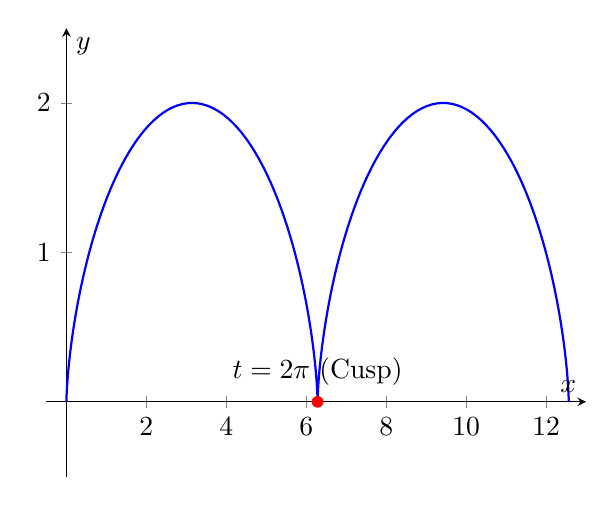
\begin{tikzpicture}
\begin{axis}[
    axis lines=middle,
    xlabel=$x$, ylabel=$y$,
    xmin=-0.5, xmax=13,
    ymin=-0.5, ymax=2.5,
    plot box ratio=0.5,
    samples=200,
    domain=0:4*pi
]
    \addplot[thick, blue] ({x - sin(deg(x))}, {1 - cos(deg(x))});
    \node[circle, fill=red, inner sep=1.5pt, label=above:{$t=2\pi$ (Cusp)}] at (axis cs:{2*pi}, 0) {};
\end{axis}
\end{tikzpicture}
\end{center}

Notice from the graph of the cycloid that at $t = 2\pi$, the curve forms a sharp sharp corner (cusp). At this point, $\vv{r}'(2\pi) = \ang{0, 0}$. Although the vector function $\vv{r}(t)$ is differentiable everywhere, the tangent line direction is undefined at the cusp because the derivative vector vanishes.

\subsection{Properties of Vector Derivatives \& Integration}

\begin{problem}{Orthogonality Property for Constant-Length Vector Functions}{implication_of_norm_r_t}
If $\norm{\vv{r}(t)} = c$ for some constant $c$, what does this imply about the relationship between $\vv{r}(t)$ and its derivative $\vv{r}'(t)$?
\end{problem}

\begin{sol}
Since $\norm{\vv{r}(t)} = c$, taking the square of both sides yields:
\[
\norm{\vv{r}(t)}^2 = c^2 \implies \vv{r}(t) \cdot \vv{r}(t) = c^2
\]
Differentiating both sides with respect to $t$ using the product rule for dot products:
\begin{align*}
\frac{\dd{}}{\dd{t}}\left(\vv{r}(t) \cdot \vv{r}(t)\right) &= \frac{\dd{}}{\dd{t}}(c^2) \\
\vv{r}'(t) \cdot \vv{r}(t) + \vv{r}(t) \cdot \vv{r}'(t) &= 0 \\
2\vv{r}(t) \cdot \vv{r}'(t) &= 0 \implies \vv{r}(t) \cdot \vv{r}'(t) = 0
\end{align*}
Therefore, $\vv{r}(t) \perp \vv{r}'(t)$ for all $t$. (The position vector is always orthogonal to its velocity vector).
\end{sol}

\subsubsection*{Product Rule Verification for Dot Products}
Given two vector-valued functions $\vv{r_1}(t), \vv{r_2}(t) \in \mathbb{R}^2$:
\begin{align*}
\frac{\dd{}}{\dd{t}}\left[\vv{r_1}(t) \cdot \vv{r_2}(t)\right] &= \frac{\dd{}}{\dd{t}}\left[x_1(t)x_2(t) + y_1(t)y_2(t)\right] \\
&= x_1'(t)x_2(t) + x_1(t)x_2'(t) + y_1'(t)y_2(t) + y_1(t)y_2'(t) \\
&= \vv{r_1}'(t) \cdot \vv{r_2}(t) + \vv{r_1}(t) \cdot \vv{r_2}'(t)
\end{align*}

\begin{problem}{Initial Value Problem for Motion}{integration_of_vector_valued_functions}
A particle moves with velocity $\vv{v}(t) = \ang{3t^2 - 2, \cos (\pi t), \sqrt{t}}$. Find its position vector $\vv{r}(t)$, given the initial condition $\vv{r}(0) = \ang{2, 1, 1}$.
\end{problem}

\begin{sol}
Integrating $\vv{v}(t)$ component-wise:
\begin{align*}
\vv{r}(t) &= \int \vv{v}(t) \, \dd{t} \\
&= \ang{\int (3t^2 - 2) \, \dd{t}, \int \cos (\pi t) \, \dd{t}, \int t^{1/2} \, \dd{t}} \\
&= \ang{t^3 - 2t + C_1, \frac{1}{\pi} \sin (\pi t) + C_2, \frac{2}{3} t^{3/2} + C_3}
\end{align*}

Applying the initial condition $\vv{r}(0) = \ang{2, 1, 1}$:
\[
\vv{r}(0) = \ang{C_1, C_2, C_3} = \ang{2, 1, 1} \implies C_1 = 2, \, C_2 = 1, \, C_3 = 1
\]
Therefore,
\[
\vv{r}(t) = \ang{t^3 - 2t + 2, \frac{1}{\pi} \sin (\pi t) + 1, \frac{2}{3} t^{3/2} + 1}
\]
\end{sol}

\textit{Note on Circular Motion:} If given acceleration $\vv{r}''(t) = \ang{-\cos t, -\sin t, 0}$, to uniquely guarantee that $\vv{r}(t)$ describes a circle centered at the origin, appropriate initial conditions for both position $\vv{r}(0)$ and velocity $\vv{r}'(0)$ must be specified.

\subsection{Arc Length of Curves}

The arc length $s$ of a smooth curve $\vv{r}(t) = \ang{x(t), y(t)}$ on $t \in [a, b]$ is derived as the limit of polygonal approximations:
\[
s = \lim_{\Delta t \to 0} \sum \sqrt{\left(\frac{\Delta x}{\Delta t}\right)^2 + \left(\frac{\Delta y}{\Delta t}\right)^2} \Delta t 
= \int_a^b \sqrt{(x'(t))^2 + (y'(t))^2} \, \dd{t} 
= \int_a^b \norm{\vv{r}'(t)} \dd{t}
\]

\begin{example}[Arc Length of a Helix]
Find the arc length of $\vv{r}(t) = \ang{\cos t, \sin t, t}$ for $t \in [0, 2\pi]$.

First, evaluate the speed $\norm{\vv{r}'(t)}$:
\[
\vv{r}'(t) = \ang{-\sin t, \cos t, 1} \implies \norm{\vv{r}'(t)} = \sqrt{(-\sin t)^2 + \cos^2 t + 1^2} = \sqrt{2}
\]
Thus, the arc length is:
\[
s = \int_0^{2\pi} \sqrt{2} \, \dd{t} = 2\pi\sqrt{2}
\]
\end{example}

\begin{example}[Arc Length of an Ellipse and Elliptic Integrals]
Consider the ellipse $x^2 + \frac{y^2}{4} = 1$.

\textbf{Method 1 (Cartesian Parameterization - Upper Half):}
Setting $x = t$ and $y = 2\sqrt{1 - t^2}$ for $t \in [-1, 1]$ yields:
\[
\vv{r}(t) = \ang{t, 2\sqrt{1 - t^2}} \implies \vv{r}'(t) = \ang{1, -\frac{2t}{\sqrt{1 - t^2}}}
\]
\[
\norm{\vv{r}'(t)} = \sqrt{1 + \frac{4t^2}{1 - t^2}} = \sqrt{\frac{1 + 3t^2}{1 - t^2}}
\]
The arc length of the upper half is given by $\int_{-1}^1 \sqrt{\frac{1 + 3t^2}{1 - t^2}} \, \dd{t}$.

\textbf{Method 2 (Trigonometric Parameterization - Full Ellipse):}
Setting $x = \cos t$ and $y = 2\sin t$ for $t \in [0, 2\pi]$:
\[
\vv{r}'(t) = \ang{-\sin t, 2\cos t} \implies \norm{\vv{r}'(t)} = \sqrt{\sin^2 t + 4\cos^2 t} = \sqrt{4 - 3\sin^2 t}
\]
The total perimeter of the ellipse is:
\[
s = \int_0^{2\pi} \sqrt{4 - 3\sin^2 t} \, \dd{t}
\]
\end{example}

\begin{definition}{Elliptic Integral}{elliptic_integral}
An elliptic integral is a type of integral that cannot be expressed in terms of elementary functions.
\end{definition}

\textit{Elliptic Integrals:} It turns out these integrals cannot be evaluated in terms of elementary functions. They belong to a class of functions known as \textbf{elliptic integrals}, which require numerical methods to evaluate.
